\section{Building Blocks}%
\label{sec:building_blocks}

Folgende Komponenten stehen zur Verfügung:
\begin{itemize}
  \item Zonen, interne oder private Netzwerke, demilitarisierte Zonen
  \item Firewalls
  \item Intrusion Detection Systems, Intrusion Prevention Systems
  \item Proxies
  \item Virtual Private Networks
\end{itemize}

\subsection{Zonen - demilitarisierte Zone}%
\label{sub:zonen_dmz}

Eine DMZ ist ein kleines Netzwerk, das öffentlich verfügbare Dienste (wie HTTP) anbietet.
Sie wird oft von einer Firewall geschützt und befindet sich außerhalb des internen
Netzwerks.
Sie wird als weniger sicher als das interne Netzwerk angesehen.

\begin{figure}[h]
  \centering
  \subcaptionbox{mit einer Firewall}{
    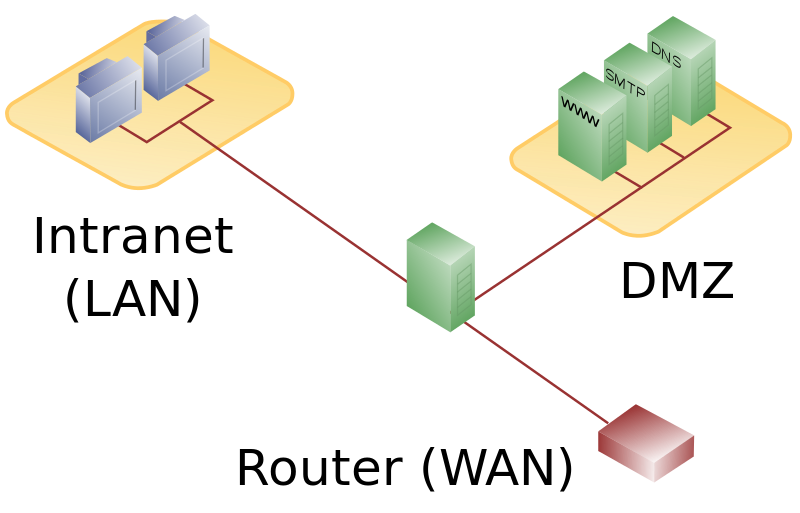
\includegraphics[width=0.4\linewidth]{bilder/dmz_1.png}
  }
  \subcaptionbox{mit zwei Firewalls}{
    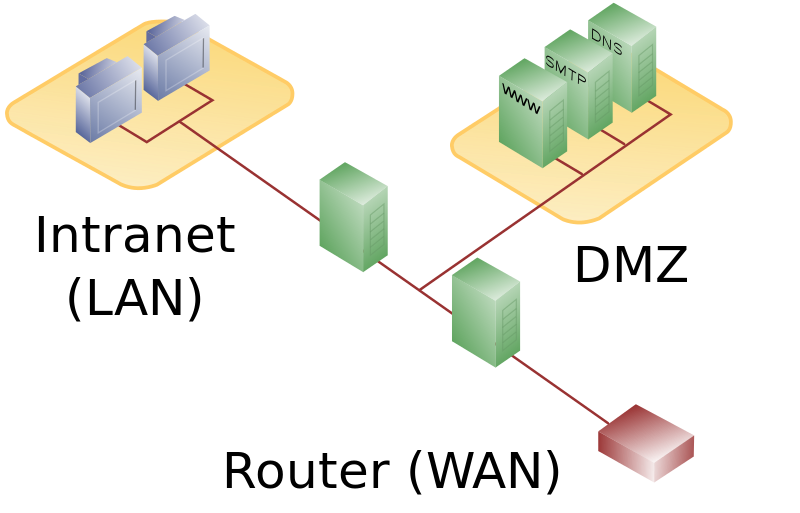
\includegraphics[width=0.4\linewidth]{bilder/dmz_2.png}
  }
  \caption{Netzwerk mit DMZ}
  \label{fig:dmz}
\end{figure}

\subsection{Internes Netzwerk}%
\label{sub:internes_netzwerk}

Schränkt den Zugang zum externen Netzwerk ein.
Der Zugang ist, wenn überhaupt, nur durch Gateways möglich.
Warum ist das nötig, wenn Angreifer sowieso nur im externen Internet sind?
Damit mögliche Schadsoftware nicht nach draußen kommunizieren kann.

Interne Angriffsrisiken hängen ab von:
\begin{itemize}
  \item Anzahl der Benutzer
  \item Vertrauen in die Nutzer
  \item Art und Weise wie die Benutzer auf das Netzwerk zugreifen
  \item Fähigkeiten der Benutzer
\end{itemize}

\subsection{Firewalls}%
\label{sub:firewalls}

Firewalls entscheiden ob Traffic passieren darf oder nicht.
Arten von Firewalls:
\begin{itemize}
  \item packet filter
  \item stateful firewalls
  \item proxy firewall
\end{itemize}

Offene Fragen bei Firewalls:
\begin{itemize}
  \item Woher kommen die Regeln?
  \item Wer entscheidet was erlaubt ist?
  \item Wer wartet die Firewall?
\end{itemize}

\subsection{Intrusion Detection Systems}%
\label{sub:intrusion_detection_systems}

Ein IDS erkennt Angriffe bzw. verdächtigen Traffic.
Es hilft dabei Firewalls aufzusetzen und zu konfigurieren.
Es ist normalerweise transparent für Benutzer und Angreifer.
Zwei wesentliche Prinzipien:
\begin{itemize}
  \item Mustererkennung
  \item Anomalieerkennung
\end{itemize}

Offene Fragen bei IDS:
\begin{itemize}
  \item Wie können Anomalien erkannt werden? Welche Klassifizierungsalgorithmen stehen zur
    Verfügung?
  \item Was macht man mit den gewonnenen Informationen?
  \item Welche Reaktionen können auf einen Alarm erfolgen?
\end{itemize}

\subsection{Proxies}%
\label{sub:proxies}

Teilen sehr stark das interne und externe Netzwerk.
Normalerweise auf dem application layer.
Verhindern, dass „bestimmte“ Informationen in das interne Netzwerk geschickt werden
(Viren, Pornos, illegale Informationen).
Verhindern, dass Informationen ins externe Netzwerk gesendet werden.
Wird oft mit anderen Systemen kombiniert (Virenfilter, Spamfilter, IDS).

Proxies sind selbst ein beliebtes Ziel für Angriffe.

\subsection{VPNs}%
\label{sub:vpns}

VPNs erzeugen einen gemeinsamen Adressbereich.
Sie schützen die Kommunikation über ein ungeschütztes Netzwerk.
Die Kommunikationspartner müssen sich gegenseitig authentifizieren.
VPNs bieten Kosteneinsparungen gegenüber festgeschalteten Verbindungen.

Offene Fragen zu VPNs:
\begin{itemize}
  \item Welche kryptographischen Verfahren werden genutzt?
  \item Wie werden Zugangstokens verwaltet?
  \item Welchen Einfluss haben VPNs auf Geschwindigkeit, Routing und andere
    Sicherheitskomponenten?
\end{itemize}
